\chapter{問題}
\label{issue}
% この研究が解く問題をシャープに記述する

本章では、サービス利用者がインターネットサービスを利用する際に利用規約を読む場面において、本研究の解決する問題について述べる。また、利用規約が読まれないことに対しての問題点や原因を明確化した後に、問題解決のための要件を述べる。

\section{利用規約の認知}
2020年に消費者庁が「デジタル・プラットフォーマーの取引慣行等に関する実態調査」の一環として、デジタル広告分野についての実態調査を行い、検索サービス及びSNSの利用者向け(消費者向け)アンケート調査を行った。この調査の結果を以下に示す。
\begin{figure}[h]
  \begin{center}
      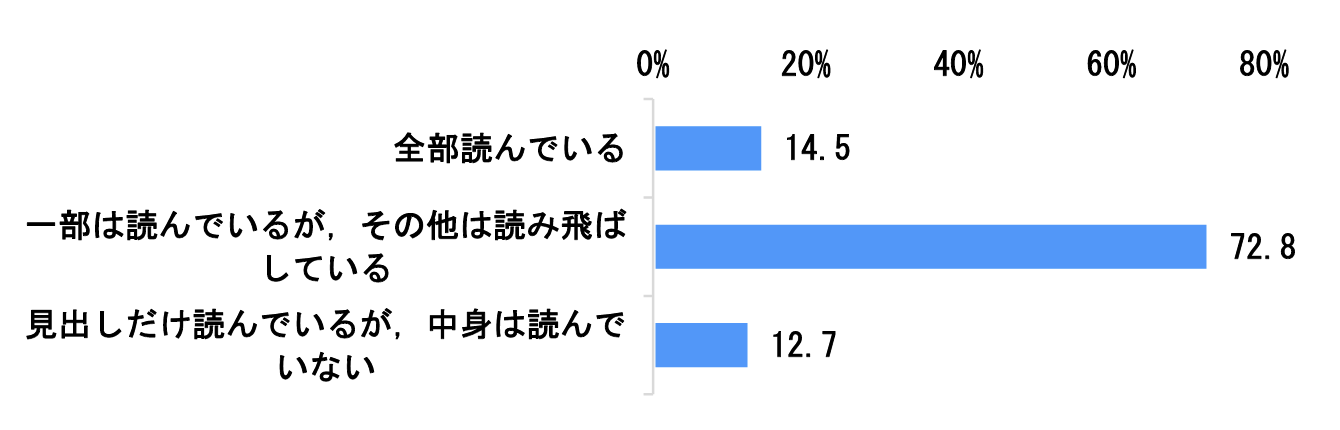
\includegraphics[width=13cm]{img/searchtosyomu.png}
      \caption{検索サービスの利用規約をどの程度読んでいるか(回答数:448)、文献\cite{jftc2021} より引用}
      \label{img:searcjtosyomu}
      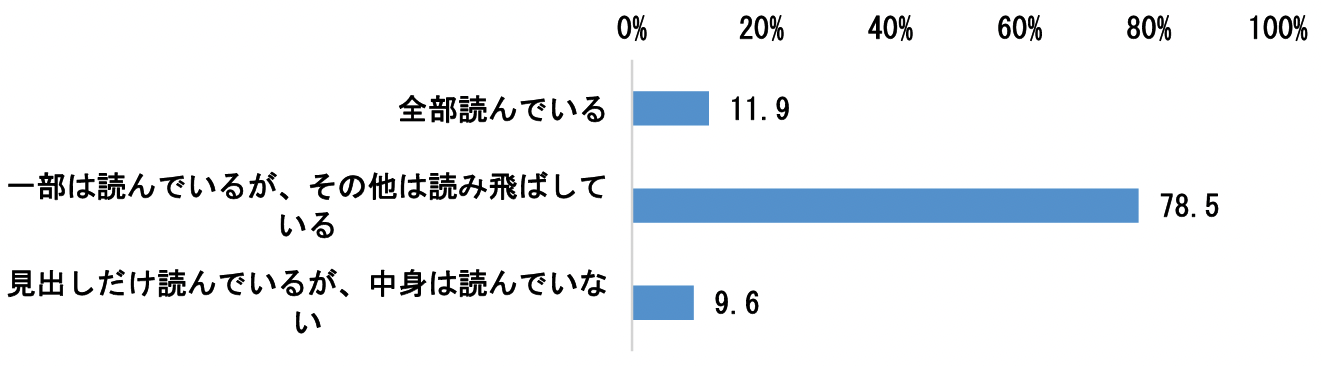
\includegraphics[width=13cm]{img/snstosyomu.png}
      \caption{SNS 等の利用規約をどの程度読んでいるか(回答数:929)、文献\cite{jftc2021} より引用}
      \label{img:snstosyomu}
  \end{center}
\end{figure}

図\ref{img:searcjtosyomu}、\ref{img:snstosyomu}では、それぞれ検索サービス、SNSについて「どの程度読んでいるか」についての調査が行われている。なお、この質問の前段では、「利用規約を認知しているか」についての質問があり、これについて「知っている」を選択した人がこの質問に回答している。このような調査では一般的に、社会適応バイアスにより高めの数値となってしまうことが多いが、それを指し引かなくとも、ほとんどの人が読み飛ばしているもしくは読んでいないという結果が示されている。

\begin{figure}[h]
  \begin{center}
      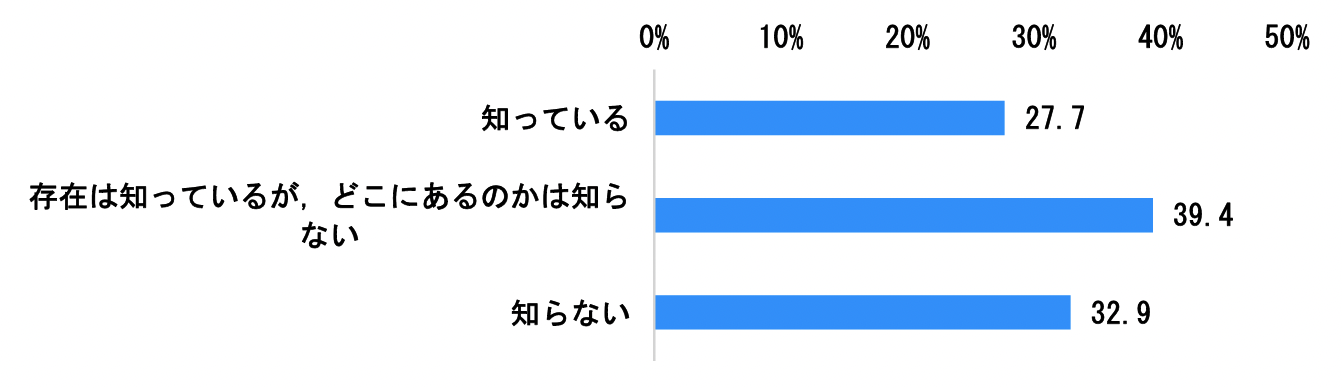
\includegraphics[width=13cm]{img/searchtosninchi.png}
      \caption{検索サービスの利用規約の認知(回答数:2,000)、文献\cite{jftc2021} より引用}
      \label{img:searchtosninchi}
      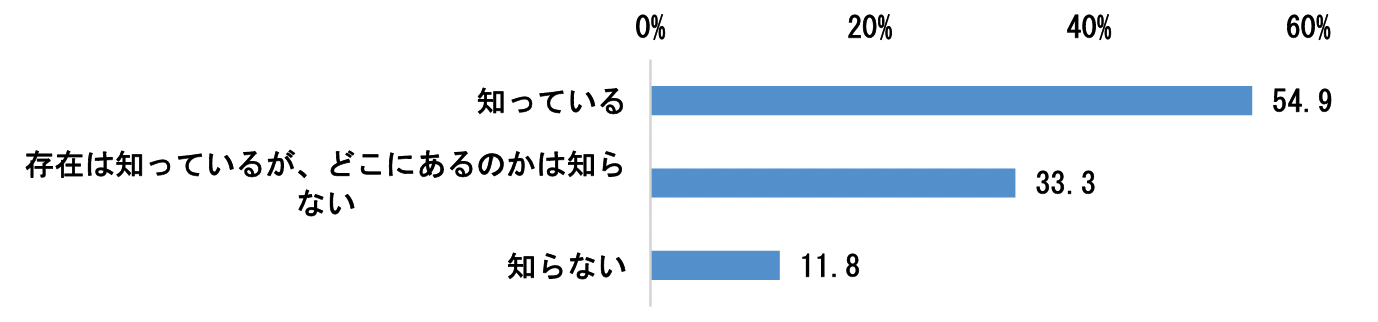
\includegraphics[width=13cm]{img/snstosninchi.png}
      \caption{SNS 等の利用規約の認知(回答数:2,000)、文献\cite{jftc2021}  より引用}
      \label{img:snstosninchi}
  \end{center}
\end{figure}

本研究では、「利用規約の認知」についてはアプローチが非常に困難であることから、この認知を前提として、「利用規約を読み飛ばしてしまう」事象を問題として定義し、それに対するアプローチについての検討を行う。

\section{利用規約の読解時間}
ネットマイル社が2012年に「ネットサービスの利用規約・プライバシー調査」を行った\cite{ネットマイル|ネ65:online}\footnote{詳細なアンケート結果はネットマイル社のサイトから削除されているため、この結果について報じている「TECH+」(マイナビ社)のニュースサイトより引用している。}。これによると、「利用規約の内容は重要だと思うか」という質問に対し、94.5\%の人が「重要だと思う」もしくは「サービスによっては重要だと思う」と答えており、利用者は利用規約に関する重要性について認識をしている(図\ref{img:toszyuuyou})。
\begin{figure}[h]
  \begin{center}
      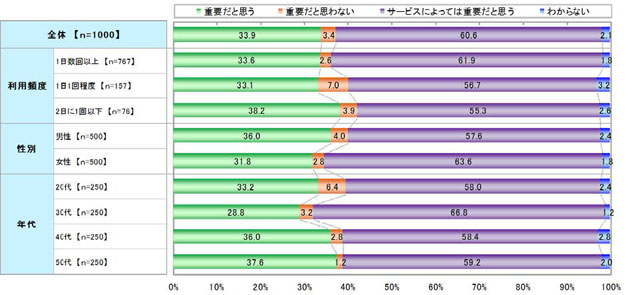
\includegraphics[width=13cm]{img/toszyuuyou.jpg}
      \caption{「利用規約の内容は重要だと思うか」、文献\cite{利用規約をきちん32:online} より引用}
      \label{img:toszyuuyou}
  \end{center}
\end{figure}
しかし、「利用規約を読まないことでリスクはあると思うか」という質問に対しては、「把握している」と答えた人は54.6\%となり重要性についての認識は重要だと思っている人の割合からは低くなっている(図\ref{img:tosrisk})。
\begin{figure}[h]
  \begin{center}
      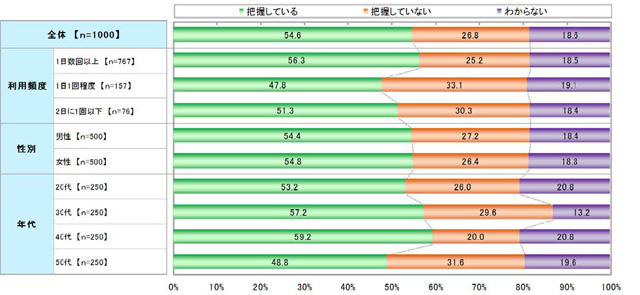
\includegraphics[width=13cm]{img/tosrisk.jpg}
      \caption{「利用規約を読まないことでリスクはあると思うか」、文献\cite{利用規約をきちん32:online} より引用}
      \label{img:tosrisk}
  \end{center}
\end{figure}
この理由の一つについて、実態として利用規約を読んでいないために具体的なリスクについて述べることができないということが考えられる。本調査においても「サービスを利用する前に利用規約を読むか」という質問がなされており(図\ref{img:tosyomuka})、読むと答えた人が15.0\%となっている。
\begin{figure}[h]
  \begin{center}
      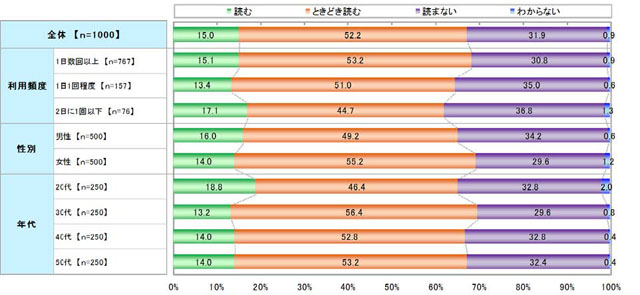
\includegraphics[width=13cm]{img/tosyomuka.jpg}
      \caption{「サービスを利用する前に利用規約を読むか」、文献\cite{利用規約をきちん32:online} より引用}
      \label{img:tosyomuka}
  \end{center}
\end{figure}
また、「利用規約を読まない理由」についても質問がなされており、全体で一番多い回答が「めんどくさい」(87.6\%)、次に「時間がない」(26.0\%)が挙げられている。
\begin{figure}[h]
  \begin{center}
      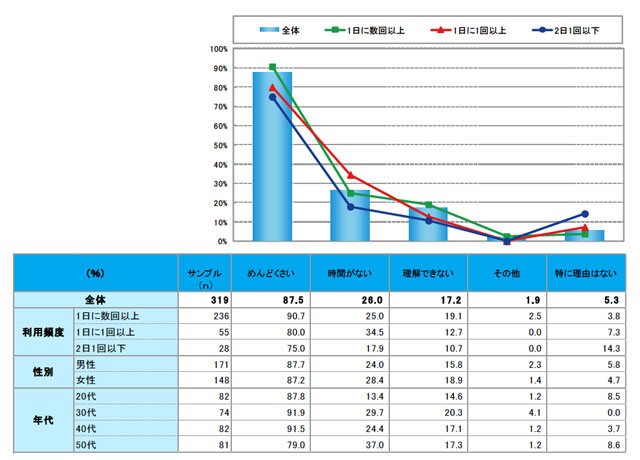
\includegraphics[width=13cm]{img/tosyomanairiyuu.jpg}
      \caption{「利用規約を読まない理由」、文献\cite{利用規約をきちん32:online} より引用}
      \label{img:tosyomanairiyuu}
  \end{center}
\end{figure}
この調査で挙げられている理由をもとにすると、利用規約を読む重要性を感じている人は多いと考えられるが、「めんどくさい」、「時間がない」などの理由により利用規約を読まないことが多いと言える。「めんどくさい」に関しては、利用規約を示す側のリスクや法的問題なども関わっており、即座に解決することは難しい。よって、本研究では、調査では次点であった「時間がない」に関してを利用規約を提示するインターネット環境においての問題点として提起する。

\section{利用規約の読解}
オムリ・ベン=シャハーほか(2022)\cite{sonokiyaku2022}は、利用規約をはじめとして、食品表示ラベル、著作権表示警告、金融機関の取引前リスク告知、医療行為の場面で行われるインフォームドコンセントなど、法令などで規制されている同意を求める行為をまとめて「開示主義」と定義し、これらの規制を「義務的情報開示」と定義している。その中で、開示主義が失敗していると述べている。(要追記)

\section{問題の定義}
利用規約を読む重要性を認識している人は多いが、その実態は利用規約を読まない人が多い。理由の一つとして、利用規約の読解のために多くの時間がかかるという点が挙げられる。このような現象により、インターネットサービスを安心して利用できる環境ではないと考えられる。よって、利用規約を読むために多くの時間がかかるということを問題定義とし、本研究では利用規約の読解時間短縮を目指す。

%先述したように、利用規約が読まれていないという問題がある。このことは、インターネット上でのサービスを利用する際に、利用規約に関して十分な理解を持っていないままサービスの利用を開始してしまうことになる。これにより、将来的に問題が発生する可能性を孕んだまま利用を継続することになる。また、利用者が利用規約この理由の1つとして、利用規約を集中して読むために必要な時間が長すぎる点が挙げられる。本研究では、そのようなユーザーに利用規約を読むことができるように利用規約の読解時間に要する時間が長いということを問題定義とする。

%\section{問題解決の要件}
